\newgeometry{top=1cm, bottom=2cm}
\section{Lineare Differentialgleichungssysteme}
\begin{figure}[h!]
    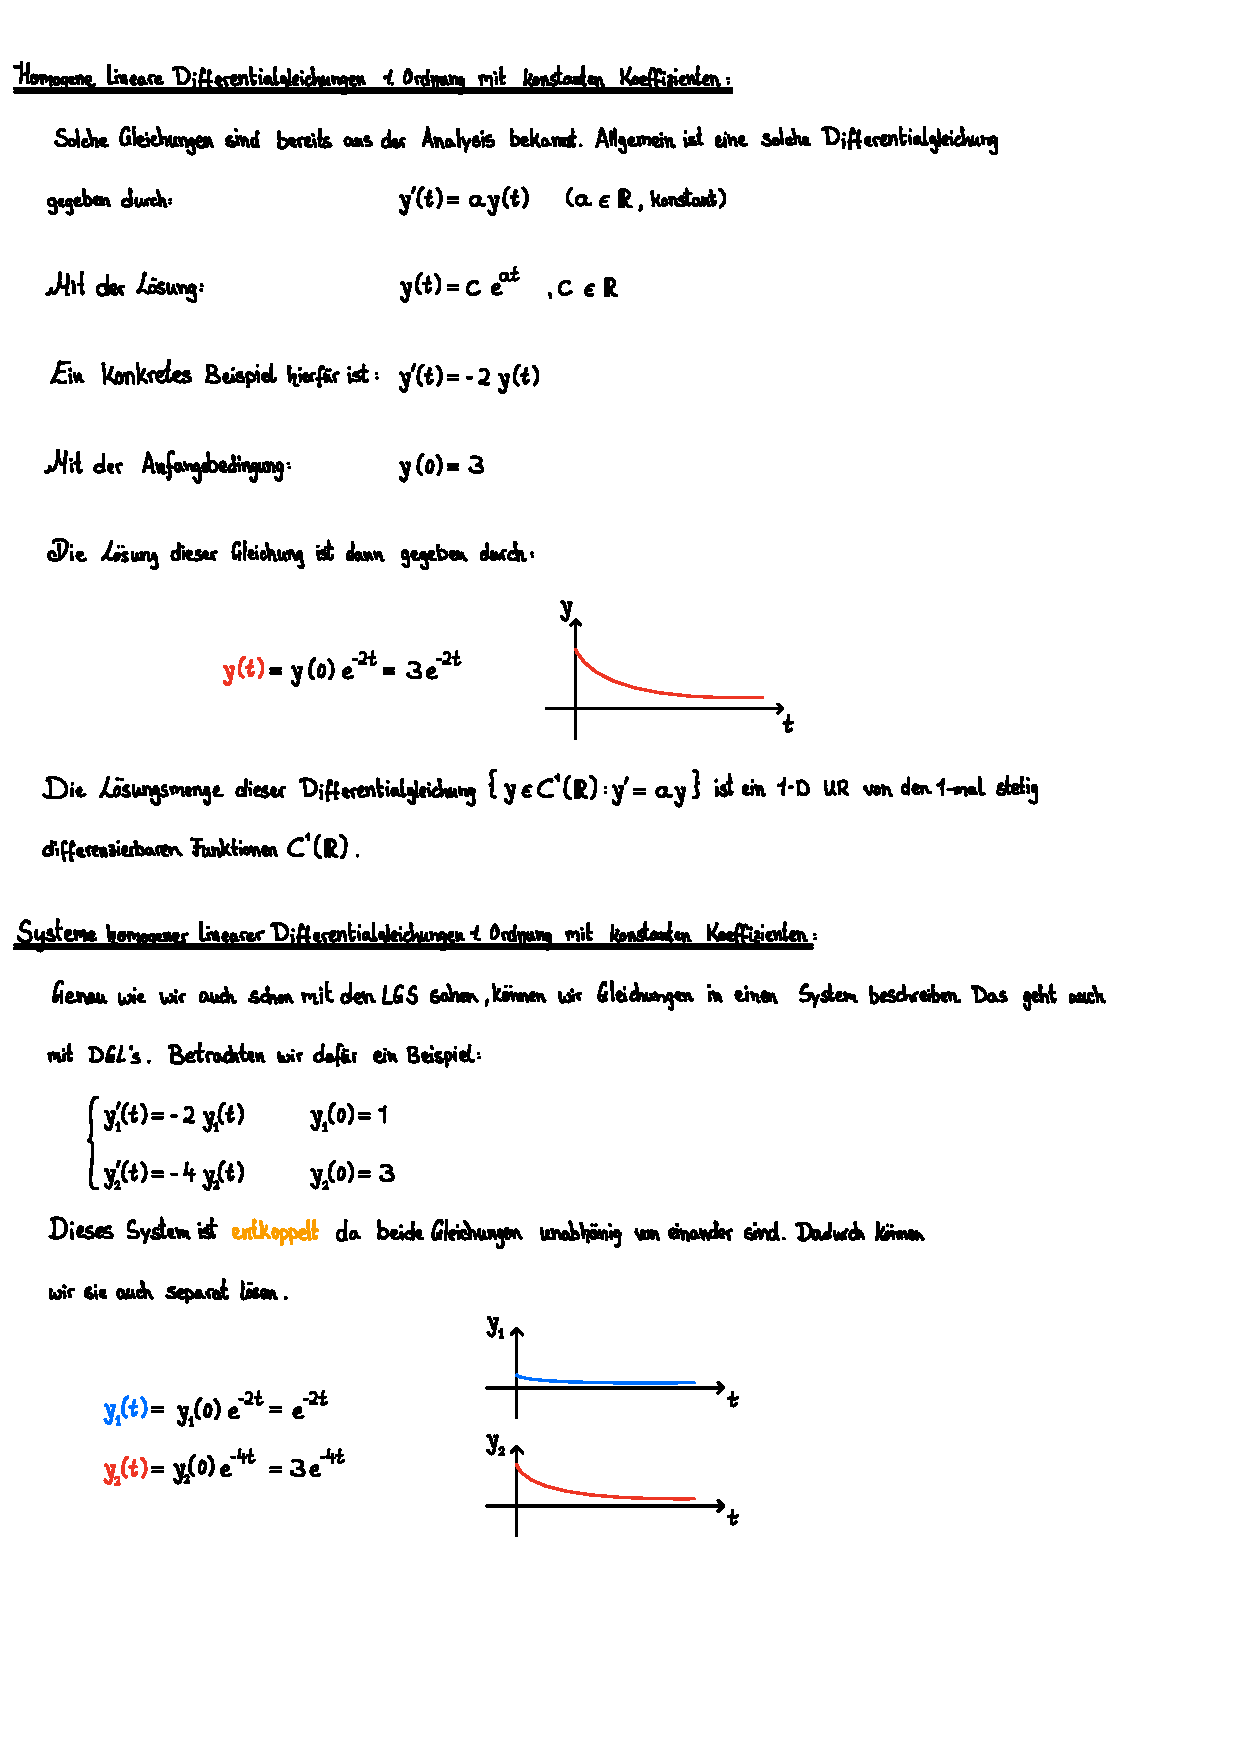
\includegraphics[page=1, scale=0.842]{pdf/08_Lineare_diff_systeme.pdf}
\end{figure}
\newpage
\includepdf[pages={2-}, 
            pagecommand={\thispagestyle{plain}}, 
            scale=0.95]{pdf/08_Lineare_diff_systeme.pdf}

\newgeometry{top=2.5cm, bottom=2cm}
\subsection{Beispielaufgaben}
\vspace{1cm}
\subsubsection{} %Zardini S. 137
Sei 
\[
A = \begin{pmatrix}
1 & 1 \\
6 & 2 \\
\end{pmatrix}.
\]
Lösen Sie das Anfangswertproblem 
\[
y'=Ay \;, \; y(0)= \begin{pmatrix}
0 \\
10 \\
\end{pmatrix}
\]
\textbf{Lösung:}

\newpage
\subsubsection{} %Übung 11 (S17)
Gegeben sei die Differentialgleichung 2. Ordnung
\begin{equation}
    y''(t) = -8y(t) + 4y'(t)  
    \tag{$\dagger$}
\end{equation}
\begin{enumerate}[label=\alph*)]
    \item Verwandeln Sie ($\dagger$) in ein Differentialgleichungssystem 1. Ordnung. Welche Dimension hat der Lösungsraum dieses Systems?
    \item Geben Sie die allgemeine reelle Lösung der Differentialgleichung ($\dagger$) an.
    \item Bestimmen Sie die Lösung von ($\dagger$) zu den Bedingungen $y(0) = 1, y(\frac{\pi}{4})=1$.
\end{enumerate}

\textbf{Lösung:}

\newpage
\subsubsection{} %Zardini S. 154
Gegeben sei das Differentialgleichungssystem 2. Ordnung
\[\begin{aligned}
y''(t) &= -2y(t) + z(t)\\
z'(t) &= -6y(t) + 3z(t)
\end{aligned}\] 
\begin{enumerate}[label=\alph*)]
    \item Verwandeln Sie das Differentialgleichungssystem in ein System 1. Ordnung. 
    \item Geben Sie die allgemeine Lösung des in a) gefundenen Systems an.
\end{enumerate} 

\textbf{Lösung:}
